%!TEX root = ../../dissertation.tex

\section{Tables and Figures}

\begin{table}[tph]
  \caption{Accuracy and speed of value iterative methods}
  \label{clmm:Table1}\vspace{-0.3cm}
  \par
  \begin{center}
  \begin{threeparttable}
{\footnotesize
  \begin{tabular}{c|cc|ccc}
    \hline \hline
    Degree & $L_1$ & $L_\infty$ & Julia CPU (s) & Matlab CPU (s) & Python CPU (s) \\ \hline
    \multicolumn{6}{c}{} \\
    \multicolumn{6}{c}{Conventional VFI (VFI)} \\ \hline
    2nd &  -3.83 & -2.76 & 2.06 & 74.02 & 11.20 \\
    3rd &  -4.97 & -3.32 & 1.79 & 49.87 & 6.83 \\
    4th &  -6.06 & -4.03 & 1.88 & 43.08 & 6.06 \\
    5th &  -7.00 & -4.70 & 3.28 & 32.48 & 4.61 \\ \hline
    \multicolumn{6}{c}{} \\
    \multicolumn{6}{c}{Envelope condition method (ECM)} \\ \hline
    2nd & -3.83 & -2.76 & 0.56 & 0.38 & 0.34 \\
    3rd & -4.97 & -3.32 & 0.35 & 0.21 & 0.24 \\
    4th & -6.06 & -4.03 & 0.57 & 0.22 & 0.27 \\
    5th & -7.00 & -4.70 & 0.63 & 0.11 & 0.15 \\ \hline
    \multicolumn{6}{c}{} \\
    \multicolumn{6}{c}{Endogenous grid method (EGM)} \\ \hline
    2nd & -3.81 & -2.76 & 1.03 & 59.89 & 4.11 \\
    3rd & -4.95 & -3.34 & 0.76 & 46.19 & 2.82 \\
    4th & -6.06 & -4.05 & 0.91 & 34.89 & 2.51 \\
    5th & -7.04 & -4.73 & 0.99 & 27.05 & 1.89 \\ \hline
  \end{tabular}%
  \begin{tablenotes}
    \item[a] $L_1$ and $L_\infty$ are, respectively, the average and maximum of
    absolute residuals across optimality conditions and test points (in $\log
    10$) units on a stochastic simulation of 10,000 observations. CPU is the
    time necessary for computing a solution (in seconds)
  \end{tablenotes}
}  % End footnote size
  \end{threeparttable}
  \end{center}
  \par
\end{table}

\begin{table}[tph]
  \caption{Accuracy and speed of policy iterative methods}
  \label{clmm:Table2}\vspace{-0.3cm}
  \par
  \begin{center}
  \begin{threeparttable}
{\footnotesize
  \begin{tabular}{c|cc|ccc}
    \hline \hline
    Degree & $L_1$ & $L_\infty$ & Julia CPU (s) & Matlab CPU (s) & Python CPU (s) \\ \hline
    \multicolumn{6}{c}{} \\
    \multicolumn{6}{c}{Conventional PI} \\ \hline
    2nd & -3.81 & -2.76 & 0.37 & 47.13 & 5.66 \\
    3rd & -4.95 & -3.34 & 1.58 & 39.30 & 5.07 \\
    4th & -6.06 & -4.05 & 2.06 & 41.83 & 5.75 \\
    5th & -7.04 & -4.73 & 3.28 & 32.54 & 4.44 \\ \hline
    \multicolumn{6}{c}{} \\
    \multicolumn{6}{c}{Envelope condition method iterrating on policy functions
    (ECM-PI)} \\ \hline
    2nd & -3.81 & -2.76 & 0.32 & 0.38 & 0.42 \\
    3rd & -4.95 & -3.34 & 0.37 & 0.15 & 0.34 \\
    4th & -6.06 & -4.05 & 0.55 & 0.24 & 0.41 \\
    5th & -7.04 & -4.73 & 0.64 & 0.11 & 0.27 \\ \hline
    \multicolumn{6}{c}{} \\
    \multicolumn{6}{c}{Envelope condition method iterating on derivative of
    value function (ECM-DVF)} \\ \hline
    2nd & -3.81 & -2.76 & 0.74 & 0.68 & 0.61 \\
    3rd & -4.95 & -3.34 & 1.12 & 0.66 & 0.65 \\
    4th & -6.06 & -4.05 & 1.62 & 0.69 & 0.75 \\
    5th & -7.04 & -4.73 & 4.05 & 0.73 & 0.81 \\ \hline
    \multicolumn{6}{c}{} \\
    \multicolumn{6}{c}{Euler equation method} \\ \hline
    2nd & -3.81 & -2.76 & 0.40 & 0.46 & 0.38 \\
    3rd & -4.95 & -3.34 & 0.37 & 0.28 & 0.27 \\
    4th & -6.06 & -4.05 & 0.53 & 0.24 & 0.25 \\
    5th & -7.04 & -4.73 & 0.77 & 0.11 & 0.12 \\ \hline
    \end{tabular}
  \begin{tablenotes}
    \item[a] $L_1$ and $L_\infty$ are, respectively, the average and maximum of
    absolute residuals across optimality conditions and test points (in $\log
    10$) units on a stochastic simulation of 10,000 observations. CPU is the
    time necessary for computing a solution (in seconds)
  \end{tablenotes}
}  % End footnote size
  \end{threeparttable}
  \end{center}
  \par
\end{table}

\begin{table}[tph]
  \caption{Accuracy and speed of a projection method for solving new Keynesian model}
  \label{clmm:Table3}\vspace{-0.3cm}
  \par
  \begin{center}
    \begin{threeparttable}
      {
      \footnotesize
        \begin{tabular}{c|cc|ccc}
          \hline \hline
          Degree & $L_1$ & $L_\infty$ & Julia CPU (s) & Python CPU (s) & Matlab CPU (s) \\ \hline
          \multicolumn{6}{c}{} \\
          \multicolumn{6}{c}{Inflation target $\pi_*=1.0598$} \\ \hline
          1st    & -3.41 &  -1.94 &           0.74 &            0.96 &            0.79 \\
          2nd    & -4.71 &  -3.13 &           3.28 &            2.24 &            2.65 \\
          3rd    & -6.07 &  -4.25 &          14.30 &            9.18 &            7.49 \\
          4th    & -6.73 &  -4.65 &          54.84 &           94.26 &           55.57 \\
          5th    & -7.00 &  -5.47 &         902.95 &         1879.04 &         1120.17 \\  \hline
          \multicolumn{6}{c}{} \\
          \multicolumn{6}{c}{Inflation target $\pi_*=1$} \\ \hline
          1st    & -3.12 &  -1.73 &           0.39 &            0.50 &            0.47 \\
          2nd    & -4.40 &  -2.77 &           1.45 &            0.98 &            1.09 \\
          3rd    & -5.71 &  -3.54 &           6.06 &            3.81 &            3.08 \\
          4th    & -6.82 &  -4.89 &          23.62 &           38.44 &           22.45 \\
          5th    & -7.01 &  -5.12 &         375.57 &          798.46 &          461.46 \\\\ \hline
          \multicolumn{6}{c}{} \\
          \multicolumn{6}{c}{Inflation target $\pi_*=1$ with ZLB} \\ \hline
          1st    & -3.12 &  -1.73 &           0.41 &            0.45 &            0.50 \\
          2nd    & -4.40 &  -2.16 &           1.45 &            0.87 &            1.06 \\
          3rd    & -5.60 &  -2.15 &           5.86 &            3.70 &            2.95 \\
          4th    & -6.17 &  -2.15 &          23.87 &           39.73 &           22.98 \\
          5th    & -6.20 &  -2.15 &         347.89 &          822.97 &          455.39 \\ \hline
        \end{tabular}
        \begin{tablenotes}
          \item[a] $L_1$ and $L_\infty$ are, respectively, the average and maximum of
          absolute residuals across optimality conditions and test points (in $\log
          10$) units on a stochastic simulation of 10,000 observations. CPU is the time
          necessary for computing a solution (in seconds)
        \end{tablenotes}
      }
    \end{threeparttable}
  \end{center}
\end{table}

\begin{figure}
  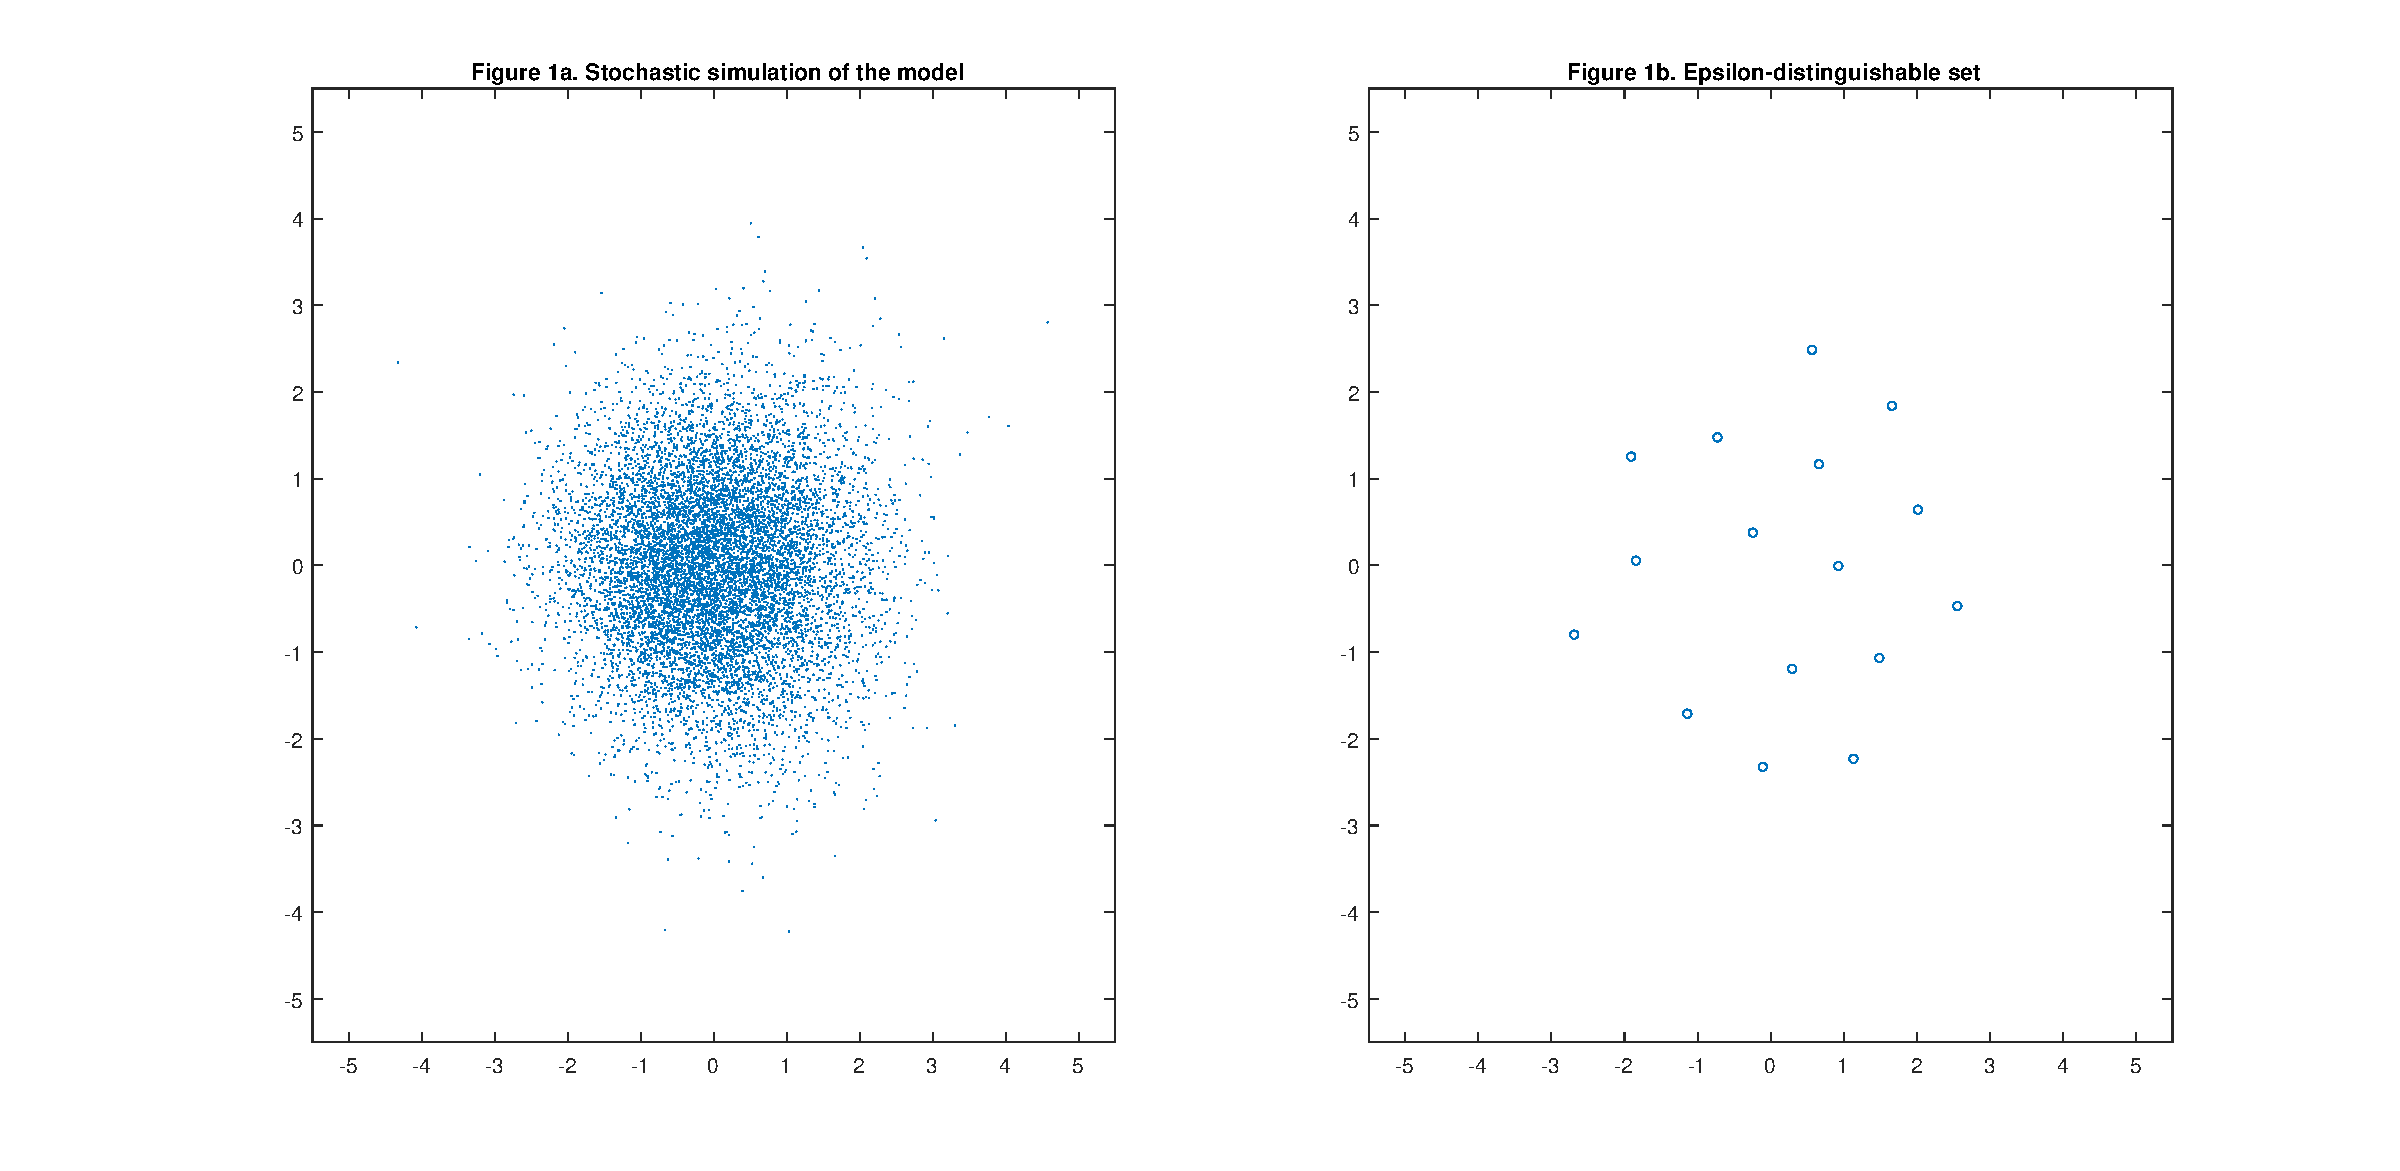
\includegraphics[width=\textwidth]{images/CLMM/Figure1-eps-converted-to.pdf}
  \caption{Stochastic-simulation grid and epsilon-distinguishable set grid. }
  \label{fig:eps_dist_grid}
\end{figure}

\begin{figure}
  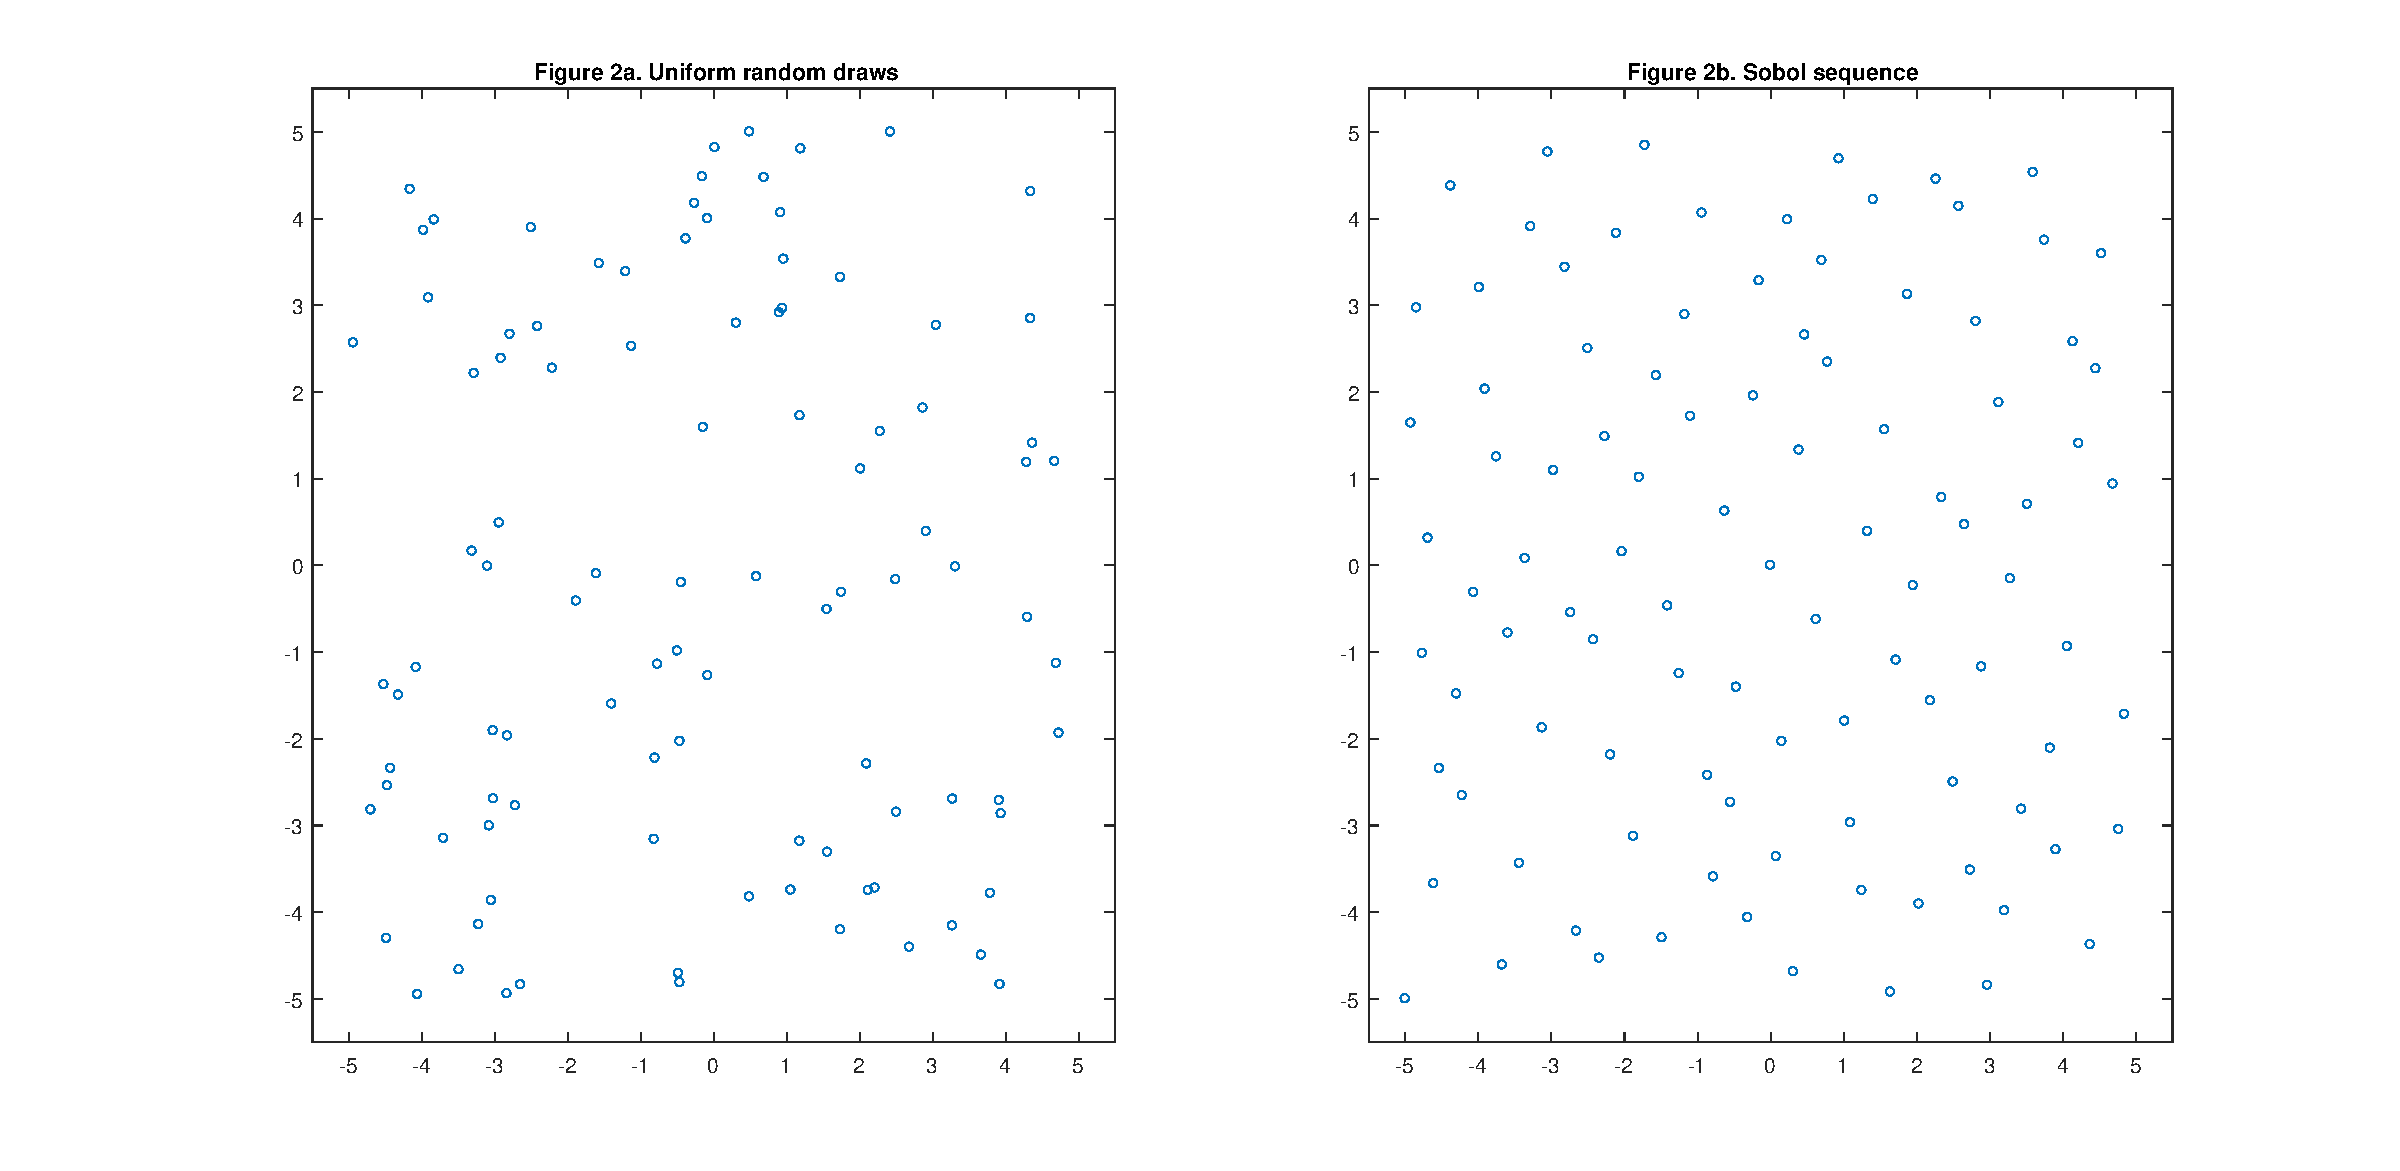
\includegraphics[width=\textwidth]{images/CLMM/Figure2-eps-converted-to.pdf}
  \caption{Uniformly-spaced random grid and quasi-Monte Carlo grid.}
  \label{fig:rand_sobol_grid}
\end{figure}
